\chapter{神经网络入门}

大家都清楚神经网络在上个世纪七八十年代是着实火过一回的,尤其是后向传播BP算法出来之后,但90年代后被SVM之类抢了风头,再后来大家更熟悉的是SVM、AdaBoost、随机森林、GBDT、LR、FTRL这些概念。究其原因,主要是神经网络很难解决训练的问题,比如梯度消失。当时的神经网络研究进入一个低潮期,不过Hinton老人家坚持下来了。\url{http://www.cnblogs.com/52machinelearning/p/5821587.html}

功夫不负有心人,2006年Hinton和学生发表了利用RBM编码的深层神经网络的Science Paper:Reducing the Dimensionality of Data with Neural Networks,不过回头来看,这篇paper在当今的实用性并不强,它的更大作用是把神经网络又推回到大家视线中,利用单层的RBM自编码预训练使得深层的神经网络训练变得可能,但那时候Deep learning依然争议很多,最终真正爆发是2012年的ImageNet的夺冠,这是后话。

ImageNet是世界图片分类大赛,下面是目前的成绩展示。\url{http://www.cnblogs.com/kuiyuan/p/4286328.html}
\begin{verbatim}
结果公布时间 	机构		top-5错误率(%) 	模型数 	方法
2015.2.11 	Google 		4.82 	  				http://arxiv-web3.library.cornell.edu/abs/1502.03167
2015.2.6 	MSRA 		4.94 	  				http://arxiv.org/abs/1502.01852
2015.2.6 	Baidu 		5.33 	  				http://arxiv.org/abs/1501.02876
2015.1.13 	Baidu 		5.98 	  				——
2014.8.18 	Google 		6.66 	  				http://arxiv.org/abs/1409.4842
2014.8.18 	Oxford 		7.33 	 			 	http://arxiv.org/abs/1409.1556
2013.11.14 	NYU 		11.7 	  				http://arxiv.org/abs/1311.2901
2012.10.13 	U.Toronto 	16.4 	  				http://www.cs.toronto.edu/~fritz/absps/imagenet.pdf
\end{verbatim}


首先从生物的大脑讲起,文章参考:\url{http://blog.csdn.net/zzwu/article/details/574931}
\section{生物学的大脑}
大脑是一块灰色的、像奶冻一样的东西。它并不像脑中的CPU那样,利用单个或少数几个处理单元来进行工作。如果你有一具新鲜地保存到福尔马林中的尸体,用一把锯子小心地将它的头骨锯开,搬掉头盖骨后,你就能看到熟悉的脑组织皱纹。大脑的外层象一个大核桃那样,全部都是起皱的[图0左],这一层组织就称皮层(Cortex)。如果你再小心地用手指把整个大脑从头颅中端出来,再去拿一把外科医生用的手术刀,将大脑切成片,那么你将看到大脑有两层: 灰色的外层(这就是“灰质”一词的来源,但没有经过福尔马林固定的新鲜大脑实际是粉红色的。如图~\ref{大脑皮层解剖图}) 和白色的内层。灰色层只有几毫米厚,其中紧密地压缩着几十亿个被称作neuron(神经细胞、神经元)的微小细胞。白色层在皮层灰质的下面,占据了皮层的大部分空间,是由神经细胞相互之间的无数连接线组成(但没有神经细胞本身,正如印刷电路板的背面,只有元件的连线,而没有元件本身那样,译注)。皮层象核桃一样起皱,这可以把一个很大的表面区域塞进到一个较小的空间里。这与光滑的皮层相比能容纳更多的神经细胞。人的大脑大约含有10G(即100亿)个这样的微小处理单元;一只蚂蚁的大脑大约也有250,000个。
\begin{figure}[H]
  \centering
  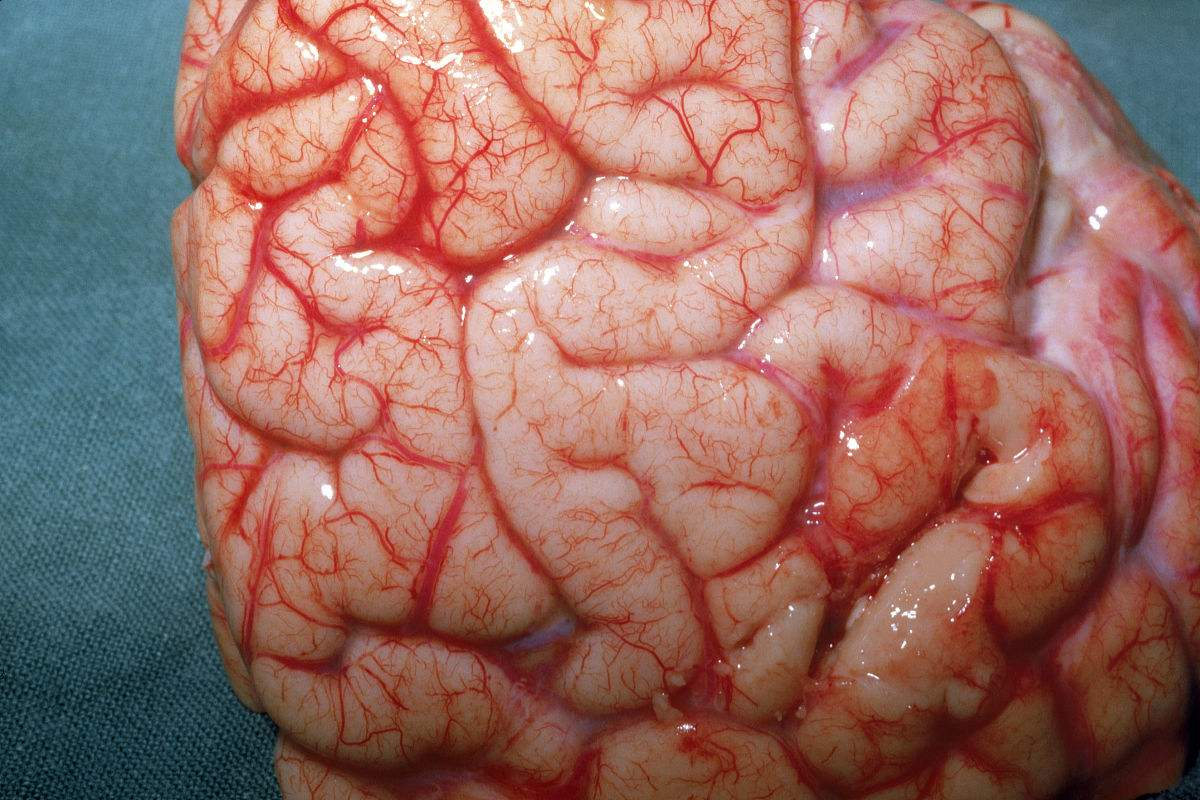
\includegraphics[width=10cm]{Figures/大脑皮层解剖图.jpg}
  \caption{大脑皮层解剖图}\label{大脑皮层解剖图}
\end{figure}

这是一个神经网络游戏的网站,很有意思。\url{http://playground.tensorflowjiaocheng.com/#JJML}